\chapter{Trabalhos Relacionados}
\label{cap:trabalhos-relacionados}

Técnicas de segmentação de imagens com o paradigma semi-supervisionado
estão em foco atualmente no campo médico, como pode ser visto em
\cite{LuoSemiSupervised2021}. Nesse artigo, uma das grandes motivações
de os autores utilizarem uma técnica semi-supervisionada
está relacionado com a dificuldade de anotação de dados no ambiente
hospitalar, requisito para utilizar técnicas mais robustas como
\textit{Mask R-CNN}.

Em relação ao tópico de redes complexas e dinâmicas coletivas, é
possível mencionar o trabalho feito com o algoritmo \gls{LCU}
\cite{VerriNetworkUnfoldingMap2018} no qual os principais conceitos
sobre resolução de problemas de aprendizagem de máquina
semi-supervisionada são explorados em detalhes como uma dinâmica de
competição de partículas na relação vértice-arestas de um grafo
não-direcionado. Este método de aprendizagem é transdutivo, portanto,
difere dos métodos indutivos, como é o caso de Redes Neurais. Além
disso, esse algoritmo tem complexidade computacional linear em relação
à quantidade de classes, arestas e vértices.

Para ilustrar uma possível ideia de segmentação de imagens, ao
considerar um algoritmo que faça uma transformação do domínio de
imagem para um grafo, é possível estabelecer uma relação na qual os
vértices representam parte da imagem como um \textit{superpixel}
\cite{SuperpixelSurvey2020}, ou seja, um grupo de subpixels da
imagem. Na Figura~\ref{fig:segmentation-superpixel} é apresentado um
exemplo de segmentação usando superpixels. Algoritmos de superpixel
são não-supervisionados em geral, portanto possuem suas limitações
quanto ao resultado esperado pelo usuário \textendash \hfill logo
difícil de ser aceito em aplicações médicas nas quais a opinião do
especialista é de alta relevância para o resultado final.

\begin{figure}[!h]
        \captionsetup{width=9cm}
		\Caption{\label{fig:segmentation-superpixel}
          Segmentação superpixel}
		\centering
		\UFCfig{}{
			\fbox{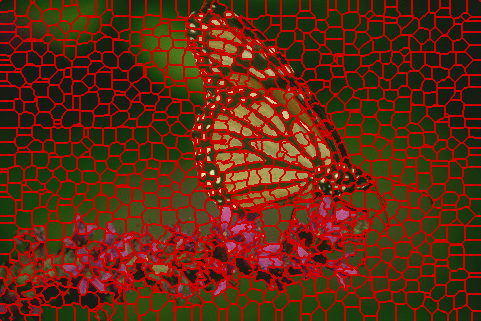
\includegraphics[width=9cm]{figuras/example-superpixel-segmentation}}
		}{
			\Fonte{\cite{SuperPixelBenchmark2017}}
		}
\end{figure}



Seguindo essa perspectiva, ao utilizar um algoritmo de extração de
\textit{features} de imagens sobre o superpixel, tem-se que o vértice
do grafo é neste momento um vetor de características. O sistema de
competição proposto no artigo \textit{Network Unfolding Map By
Vertex-Edge Dynamics Modeling} pode otimizar o pertencimento de
classes (segmentos, nesse caso) baseado na topologia de sua vizinhança
e na relação aos vértices conectados. A métrica de similaridade
(por exemplo, distância euclidiana, cosseno, etc.) pode ser
ajustada de acordo com o problema.

Ao considerar o problema como semi-supervisionado, a pista de ter
alguns dos superpixels anotados adicionaria um \textit{bias}
parametrizado pelo conhecimento do especialista em uso da ferramenta,
como um editor ou um médico. A otimização do pertencimento das classes
então seria acionada pela dinâmica coletiva selecionada em questão,
que, por acaso, poderia ser o algoritmo \gls{LCU} mencionado anteriormente.

Por outro lado, ainda há muitas melhorias a serem feitas nessas técnicas, como,
por exemplo: analisar as condições de convergência do algoritmo. Isso
pode ser um dos resultados deste trabalho, demandando uma análise
matemática com auxílio de experimentos.

É importante mencionar que já foi demonstrado em outras situações,
como em \cite{JarbasComplexNetworks2020}, que o uso de redes complexas
em fusão com redes neurais aleatórias pode gerar um discriminante de
textura da imagem de alta relevância como extrator de
características. Neste caso, é possível se apoiar nesse resultado como
uma evidência de que a investigação de novas técnicas considerando a
topologia da imagem através de redes complexas é uma oportunidade de
pesquisa.


\section{Aplicação de Agrupamento Semissupervisionado para Segmentação
de Imagens Coloridas}
\label{sec:franciscolira2018}

Neste trabalho o autor \cite{franciscolira2018}, na sua tese de
graduação, propõe variações de um algoritmo de segmentação de imagem
semi-supervisionado combinando algoritmos de agrupamento, como
\textit{Fuzzy C-Means}, Algoritmo de Pedrycs, Algoritmo
Semi-supervisionado Padrão (sSSC) e Algoritmo Semi-supversionado
Regularizado por Entropia (ESSC).


% LocalWords:  transdutivo superpixel
